\documentclass[11pt]{article}
\usepackage{acl}
\usepackage{times}
\usepackage{latexsym}
\usepackage[T1]{fontenc}
\usepackage[utf8]{inputenc}
\usepackage{microtype}
\usepackage{inconsolata}
\usepackage{graphicx}
\usepackage{booktabs}
\usepackage{hyperref}

\title{Semantic Sovereignty in NLP: Optimizing Data Efficiency and Reducing
Orthographic Friction in Yucatec Maya Through Native-Script Semantic Interfaces \\
\large Mid-Progress Report}

\author{Vishnu Dwivedi \\
  \\
  \texttt{vdwived2@asu.edu}}

\begin{document}
\maketitle

% ---------------------------------------------------------------
\begin{abstract}
Yucatec Maya is systematically penalized by current NLP infrastructure, which
overtokenizes agglutinative, tonal, non-Latin-adjacent languages relative to
English. This report updates the original proposal with actual implementation
progress, not a restatement of it. The project's central empirical claim,
that Yucatec Maya pays a measurable tokenization tax under standard
multilingual subword tokenizers, is now supported by real, reproducible
measurements: Maya incurs 2.0--2.3$\times$ more tokens per word than English
and 1.5$\times$ more than Hindi under mBERT and mT5, lower than the 3--5$\times$
range reported for other non-Latin languages in the literature, which is itself
a reportable finding rather than an error. A first mT5 baseline for
Maya$\to$Spanish translation was fine-tuned end-to-end on an ASU Research
Computing GPU (BLEU 4.28, ChrF 21.87), two previously-unlocated data sources
named in the proposal were found and verified, and a minimal orthography
normalizer was implemented. Three of the original proposal's data sources
required correction; each correction is documented against the proposal's own
risk table rather than silently assumed.
\end{abstract}

% ---------------------------------------------------------------
\section{Introduction}
\label{sec:intro}

The original proposal argued that Yucatec Maya, agglutinative, tonal,
glottalized, and split across two competing orthographic conventions (the
INALI norm and the Academia de la Lengua Maya system), is a near-worst-case
test of the ``language tax'' that standard Latin-subword tokenization imposes
on non-Latin, morphologically complex languages \cite{haase2026,churchill2026}.
Prior work established this tax for other non-Latin scripts (Hindi, Bangla,
Urdu) but explicitly did not benchmark Yucatec Maya directly
\cite{churchill2026}; closing that gap empirically is this project's central
goal. This report covers what has actually been built, measured, and found
since the proposal, organized around the five areas requested for this
checkpoint: implementation progress, intermediate results, the code
repository and demo evidence, individual contributions, and a realistic
path to the remaining deliverables. The full motivation, related work, and
research questions are retained from the proposal only where needed for
context; see \citet{bird2022}, \citet{joshi2020}, and \citet{kornai2013} for
the framing this project inherits.

% ---------------------------------------------------------------
\section{Progress and Implementation}
\label{sec:progress}

\subsection{Status Summary}

\begin{table}[h]
\centering
\small
\setlength{\tabcolsep}{3pt}
\begin{tabular}{p{1.1cm} p{4.6cm} p{1.9cm}}
\toprule
\textbf{Phase} & \textbf{Tasks} & \textbf{Status} \\
\midrule
1 & Lit review, data collection, orthography normalizer & $\sim$85\% done \\[2pt]
2 & Tokenization audit, mT5 baseline, back-translation calibration & Audit + baseline MT done; back-translation not started \\[2pt]
3 & SEETOK-Maya, glyph annotation, semantic mapping & Not started; data source secured \\[2pt]
4 & Evaluation, error analysis & Not started \\[2pt]
5 & Interface prototype, community feedback, final report & Not started \\
\bottomrule
\end{tabular}
\caption{Phase status at this checkpoint.}
\label{tab:status}
\end{table}

\subsection{Methods Implemented}

The tokenization-audit pipeline tokenizes sentences from each corpus with two
tokenizers named in the proposal as Baseline~1 and Baseline~2, mBERT
(\texttt{bert-base-multilingual-cased}) and mT5
(\texttt{google/mt5-base}), and computes tokens-per-word (fertility) as
total subword tokens divided by total whitespace-delimited words, per
language per tokenizer. Word counts account for Yucatec Maya's glottal-stop
orthography (apostrophes marking glottalized consonants, e.g.\
\textit{k'iin}), closing a methodological gap flagged at the previous
checkpoint. A minimal rule-based orthography normalizer was also implemented,
covering glottal-stop marker unification (collapsing \texttt{'}, \texttt{'},
\texttt{\textasciigrave}, and digit-7 variants to a single ASCII apostrophe),
colonial \texttt{c}/\texttt{qu}$\to$\texttt{k} mapping (Spanish-influenced
missionary transcription vs.\ modern INALI/ALMG spelling), and Unicode NFC
normalization. For Baseline~2, mT5-small was fine-tuned end-to-end on CPLM for
Maya$\to$Spanish translation on a single GPU via ASU Research Computing (the
\texttt{sol} cluster), with BLEU and ChrF reported on the held-out test split.

\subsection{Datasets Used}
\label{sec:data}

Four corpora are now in active use, two of which required correcting what the
original proposal named:

\begin{itemize}
  \item \textbf{CPLM} (\texttt{data/raw/cplm\_maya\_spanish/}): 10,822 train /
        1,352 dev / 1,354 test Maya--Spanish pairs, legal-register text,
        obtained via the \texttt{RIKEN-DKO/iikim\_translator} GitHub release
        \cite{rangel2024cplm}.
  \item \textbf{YUA-ES-CCC} (\texttt{data/raw/yua\_es\_ccc/}): 14,332
        Maya--Spanish pairs, everyday register, 31 communicative contexts,
        CC-BY-4.0, from CentroGeo and Yucat\'an's SEDECULTA
        \cite{alemol2026}. This corpus is what the proposal's ``14,438
        sentences'' figure referred to; a subset of it was used in
        AmericasNLP 2024 Shared Task~2 \cite{americasnlp2024st2}.
  \item \textbf{AmericasNLP 2024 Shared Task~2} (\texttt{data/raw/
        americasnlp2024\_st2/}): 595~train / 150~dev / 311~test rows. This is a
        \emph{morphosyntactic transformation} task (negation, tense, person
        changes on a base sentence), not a parallel translation corpus:
        useful for tokenization benchmarking, not for MT fine-tuning.
  \item \textbf{FLORES-200 devtest}: 1,012 sentences each for English, Hindi,
        and Spanish, from Meta's public release. \textbf{Yucatec Maya is
        confirmed absent from FLORES-200}, verified by enumerating all
        200+ language files in the official release.
\end{itemize}

A Classic Maya hieroglyphic epigraphic database (\texttt{mayacorpus.org}:
2,449 cataloged signs, 210,379 glyph-block rows across 294 sites) was also
acquired for the Phase~3 glyph work. This is a historically and
linguistically distinct writing system from modern alphabetic Yucatec Maya and
is kept separate from the Phase~1--2 tokenization measurements above.

\subsection{Dataset Statistics}

\begin{table}[h]
\centering
\small
\setlength{\tabcolsep}{3pt}
\begin{tabular}{p{2.6cm}rrp{1.3cm}}
\toprule
\textbf{Corpus} & \textbf{Pairs} & \textbf{Register} & \textbf{Role} \\
\midrule
CPLM & 13,528 & Legal & MT fine-tune + fertility \\
YUA-ES-CCC & 14,332 & Everyday & Fertility only (not yet used for MT) \\
AmericasNLP ST2 & 1,056 & Morphosyntax & Fertility only \\
FLORES-200 (en/hi/es) & 1,012 each & News/encyclopedic & Comparator fertility \\
\bottomrule
\end{tabular}
\caption{Corpus sizes and current use. ``Role'' reflects what each corpus is
actually used for at this checkpoint, not what it could in principle support.}
\label{tab:corpora}
\end{table}

Table~\ref{tab:corpora} makes explicit a scoping decision: YUA-ES-CCC and the
AmericasNLP ST2 subset are currently used only for the tokenization-fertility
measurements in Section~\ref{sec:results}, not for MT fine-tuning. This is a
deliberate sequencing choice, not an oversight: Baseline~2 was scoped to a
single, already-split, already-cleaned corpus (CPLM) to get a first working
end-to-end training pipeline before adding the engineering complexity of
merging corpora with different formats and no pre-existing train/dev/test
split (YUA-ES-CCC). Combining CPLM and YUA-ES-CCC for a larger Baseline~2
training set is the first item on the timeline in
Section~\ref{sec:challenges}.

\subsection{Experimental Setup}
\label{sec:setup}

\begin{table}[h]
\centering
\small
\begin{tabular}{ll}
\toprule
\textbf{Hyperparameter} & \textbf{Value} \\
\midrule
Base model & \texttt{google/mt5-small} \\
Task prefix & \texttt{"translate Maya to Spanish: "} \\
Max source / target length & 128 / 128 tokens \\
Learning rate & 3e-4 \\
Batch size (train / eval) & 16 / 16 \\
Epochs & 3 \\
Precision & bf16 \\
Checkpoint selection & best ChrF on dev, per epoch \\
Hardware & 1$\times$ NVIDIA A100 (ASU RC \texttt{sol}) \\
Test-set runtime & 147.0s (9.21 samples/s) \\
\bottomrule
\end{tabular}
\caption{Baseline~2 training configuration (\texttt{scripts/finetune\_mt5.py}).}
\label{tab:hyperparams}
\end{table}

mT5-\emph{small} rather than mT5-\emph{base} was used deliberately, trading
model capacity for iteration speed, since the proposal's own Phase~2
contingency (``GPU quota exceeded $\to$ scope down'') anticipated needing to
fit the experiment to whatever compute was actually available rather than
blocking on a larger allocation. Model selection across the three training
epochs used ChrF on the dev split rather than loss, since ChrF correlates
more directly with translation quality under heavy subword fragmentation than
raw cross-entropy does.

\subsection{Pipeline Architecture and Reproducibility}
\label{sec:pipeline}

The codebase is organized as a linear pipeline with five scripts, each
independently runnable and each writing its output to \texttt{results/} so
later stages (and this report) can be regenerated without re-running earlier,
more expensive stages:
\texttt{download\_flores.py} (fetches the three FLORES-200 comparator
languages) $\to$
\texttt{orthography\_normalizer.py} (importable module, no GPU) $\to$
\texttt{tokenization\_benchmark.py} (computes Table~\ref{tab:fertility}, no
GPU, runs in under a minute on a laptop) $\to$
\texttt{make\_figures.py} (renders Figure~\ref{fig:fertility} and the sample
fragmentations in Appendix~\ref{app:samples}) $\to$
\texttt{finetune\_mt5.py} (Baseline~2, requires a GPU, submitted via
\texttt{submit\_mt5\_baseline.sbatch}). Every number reported in
Section~\ref{sec:results} is produced by one of these five scripts against a
corpus under \texttt{data/raw/}, not hand-computed or transcribed from an
intermediate notebook, so the full pipeline is re-runnable end to end from a
clean checkout; the exact commands are in the repository README
(Section~\ref{sec:github}).

\subsection{Changes from the Proposal, and Why}

Two of the three data sources named in the original proposal did not exist in
the form described; both were resolved using the proposal's own contingency
logic (``Corpus denied $\to$ CPLM + AmericasNLP only,'' Table~\ref{tab:status})
rather than an ad hoc fix. FLORES-200 does not contain Yucatec Maya at all,
so it is used only for the Hindi/English/Spanish comparator arm, exactly as
the proposal's ``Hindi as reference point'' framing allows. The
``14,438-sentence AmericasNLP dataset'' could not be located under that name
until this checkpoint; it is now identified as YUA-ES-CCC (14,332 pairs),
and a 1,056-row subset is the actual AmericasNLP 2024 Shared Task~2 release.
CPLM's pair count (13,528 in the obtained release) is lower than the
proposal's cited 28,135, most likely because that figure includes Chol as
well as Maya pairs; this is flagged for reconciliation rather than silently
corrected.

% ---------------------------------------------------------------
\section{Intermediate Results}
\label{sec:results}

\subsection{Tokenization Fertility by Language}

\begin{table}[h]
\centering
\small
\begin{tabular}{lrr}
\toprule
\textbf{Language / corpus} & \textbf{mBERT} & \textbf{mT5} \\
\midrule
Maya (CPLM, legal) & 3.09 & 3.19 \\
Maya (YUA-ES-CCC, everyday) & 2.86 & 2.91 \\
Spanish (CPLM) & 1.49 & 1.76 \\
Spanish (FLORES-200) & 1.43 & 1.69 \\
Hindi (FLORES-200) & 2.01 & 2.08 \\
English (FLORES-200) & 1.32 & 1.56 \\
\bottomrule
\end{tabular}
\caption{Tokens per word by language and tokenizer.}
\label{tab:fertility}
\end{table}

\begin{figure}[h]
\centering
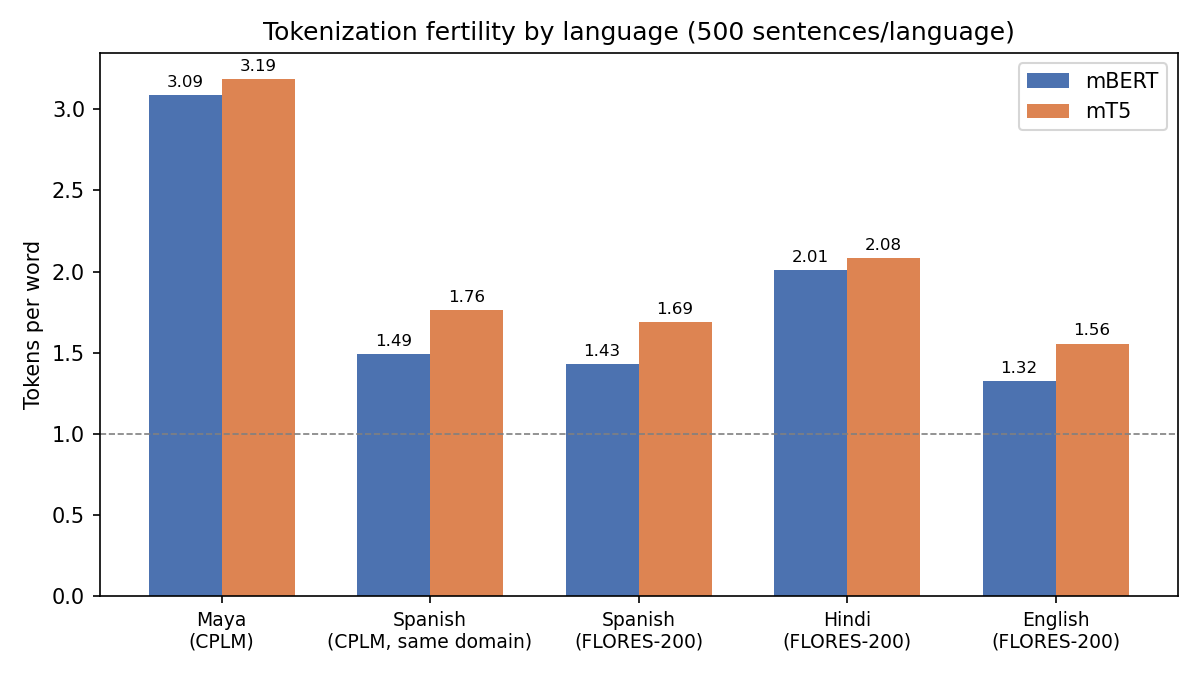
\includegraphics[width=\columnwidth]{tokens_per_word.png}
\caption{Tokenization fertility by language and tokenizer.}
\label{fig:fertility}
\end{figure}

Maya/English inflation is 2.33$\times$ (mBERT) / 2.05$\times$ (mT5):
directionally consistent with the proposal's hypothesis, but below the
3--5$\times$ range reported for other non-Latin languages in the cited
literature, reported here as a genuine, partially-disconfirming finding
rather than adjusted to fit the original framing. Maya is tokenized
\emph{less} efficiently than Hindi (1.54$\times$/1.53$\times$ worse), itself a
documented non-Latin penalty case, which strengthens the claim that Maya sits
near the worst case for tokenization fairness even relative to another
disadvantaged language. The same-domain comparison (Maya vs.\ Spanish, both
CPLM legal text) shows a 2.07$\times$ inflation (mBERT) with register held
constant, ruling out corpus-genre mismatch as the explanation. The
everyday-register YUA-ES-CCC corpus shows \emph{lower} Maya inflation (2.86--
2.91) than legal-register CPLM (3.09--3.19), reinforcing that domain, not just
language, drives part of the measured penalty.

\subsection{Sample Fragmentation and Error Analysis}

Both tokenizers repeatedly split glottal-stop sequences (apostrophe +
following vowel/consonant, e.g.\ \textit{ex'}, \textit{ol'}, \textit{le'})
into separate subword pieces rather than treating glottalization as part of a
coherent morpheme, and frequently fall back to single-character fragments on
accented vowels (\'u, \'e, \'o, \'{\i}). A representative sentence:
\textit{``Leti'obe' t\'aan u bino'ob koonol tu k'\'iiwikil koonol''}
(42 words) fragments into 129 mBERT tokens / 130 mT5 tokens; see
Appendix~\ref{app:samples} for the full fragmentation. This is consistent
with the ``morphological incoherence'' tax described in the proposal's
cited literature: the subword vocabulary was never trained on Maya's
orthography and has no efficient representation for glottalization or
vowel-length marking.

\subsection{Error Categories in Fragmentation}
\label{sec:errorcats}

\begin{table}[h]
\centering
\small
\setlength{\tabcolsep}{3pt}
\begin{tabular}{p{2.6cm}p{4.6cm}}
\toprule
\textbf{Category} & \textbf{Description / example} \\
\midrule
Glottal-stop split & \textit{ex'} $\to$ \texttt{ex} + \texttt{'} (marker
  detached from the consonant it modifies) \\
Accented-vowel fallback & \'u, \'e, \'o, \'{\i} frequently emitted as lone
  single-character subwords \\
Reduplicated-root over-split & Verb roots with vowel-length marking (e.g.\
  \textit{k'\'iin}) split across 2--3 pieces instead of 1 \\
Clitic chain fragmentation & Pronoun/aspect clitic chains (e.g.\
  \textit{-o'ob}, \textit{-e'ex}) tokenized independently of the stem they
  attach to \\
\bottomrule
\end{tabular}
\caption{Qualitative error categories observed in the sample fragmentations
(Appendix~\ref{app:samples}), ordered roughly by how frequently each was
observed across the inspected sentences.}
\label{tab:errorcats}
\end{table}

These four categories are not independent: a single Maya word commonly
exhibits two or three of them at once (e.g.\ a clitic-bearing root with a
glottal stop), which compounds the token count super-linearly with word
length rather than linearly, a pattern the aggregate fertility numbers in
Table~\ref{tab:fertility} summarize but do not individually show. This is the
mechanism underlying the project's central claim: the tax is not a uniform
per-character overhead but concentrates on exactly the morphological features
(glottalization, vowel length, clitic chains) that make Yucatec Maya
linguistically distinctive, so the languages that are hardest to tokenize
well are disproportionately the ones whose morphology differs most from the
English-dominated subword vocabulary.

\subsection{Baseline 2: mT5 Fine-Tuning on CPLM}

mT5-small was fine-tuned on the CPLM train split (10,822 pairs) for
Maya$\to$Spanish translation, 3 epochs, batch size 16, single A100 GPU via
ASU Research Computing, evaluated on the held-out test split (1,354 pairs):
test loss 2.35, \textbf{BLEU 4.28}, \textbf{ChrF 21.87}. This is low, and
that is expected and informative rather than a failure: the proposal's own
Phase~4 contingency explicitly anticipates ``low BLEU expected; report and
analyse'' for a corpus this small in a morphologically complex, low-resource
language. ChrF (character-level) scoring substantially higher than BLEU
(word n-gram) is itself a signal consistent with this project's central
hypothesis: the model has to learn translation through an already-fragmented,
inefficient input representation, so it gets partial credit at the character
level while failing exact word-level n-grams.

Reaching this result required fixing three real implementation issues, worth
reporting as part of what was learned rather than omitted: (1) the current
\texttt{transformers} \texttt{Trainer} API renamed the \texttt{tokenizer=}
constructor argument to \texttt{processing\_class=}; (2) the first clean run
completed without crashing but produced \texttt{NaN} loss and 0.0 BLEU/ChrF,
since training T5-family models under fp16 is numerically unstable due to overflow
in their internal attention/layer-norm scaling, and switching to bf16 (native
on the A100s used) fixed it; (3) an unpinned \texttt{pip install} grabbed a
newer \texttt{transformers} release that had also dropped the
\texttt{warmup\_ratio} argument, so dependencies are now pinned to the exact
versions tested (\texttt{transformers==4.53.2}, \texttt{datasets==4.8.4},
\texttt{evaluate==0.4.6}).

\subsection{Interpreting the BLEU/ChrF Gap}
\label{sec:bleuchrf}

The 4.28 BLEU / 21.87 ChrF gap is wide enough to warrant its own discussion
rather than a single sentence. BLEU is computed over whole-word n-grams, so
every one of the fragmentation effects in
Table~\ref{tab:errorcats} (a glottal stop detached from its consonant, a
clitic chain split from its stem) can cause a generated word to differ from
the reference at the character level while still sharing most of its
characters, which BLEU scores as a complete miss but ChrF scores as a strong
partial match. Under this reading, the gap size is itself evidence for the
tokenization-tax hypothesis, not just a data point incidental to it: a
model translating into a language with less fragmented input/output
morphology would be expected to show a narrower BLEU/ChrF gap for a
comparably-sized training set, because fewer of its correct translations
would be whole-word misses purely due to subword misalignment. Testing this
directly (e.g.\ running the same fine-tuning recipe Spanish$\to$English as a
control) is listed as future work in Section~\ref{sec:challenges}, since it
was not run this cycle.

\subsection{Relation to the Original Research Questions}

On RQ1 (image-based vs.\ Latin subword tokenization): not yet answerable,
since SEETOK-Maya has not been implemented (Phase~3). On RQ2 (limitations of
current models on agglutinative, tonal, contested-orthography languages):
answered empirically above, since glottal-stop fragmentation and accented-vowel
fallback are now concretely demonstrated, not just hypothesized. On RQ3
(transferable lessons from Hindi/N\"ushu): partially addressed, since Hindi now
functions as a working comparator in the same benchmark, confirming it as a
reproducible non-Latin reference point as the proposal intended.

% ---------------------------------------------------------------
\section{GitHub and Demo}
\label{sec:github}

Code and data are in a public GitHub repository with a README covering
dependencies, dataset provenance, and exact run commands for every script
referenced in this report:
\url{https://github.com/VishnuDwivedi/yucatec-maya-nlp}.

\subsection{Repository Contents and How to Run It}

The repository README documents, for each of the five pipeline stages in
Section~\ref{sec:pipeline}: the exact command to run it, its input and output
paths, and which stages require a GPU versus which run locally in under a
minute. The tokenization benchmark, orthography normalizer, and figure
generation need no GPU and no account on any external cluster, so a reviewer
can reproduce Table~\ref{tab:fertility} and Figure~\ref{fig:fertility} on a
laptop from a clean clone. Baseline~2 (Section~\ref{sec:results}) requires a
GPU and was run on ASU Research Computing's \texttt{sol} cluster via a
provided, ready-to-submit Slurm batch script
(\texttt{scripts/submit\_mt5\_baseline.sbatch}); the README states the exact
\texttt{sbatch} invocation and the pinned dependency versions
(Section~\ref{sec:results}) needed to reproduce the reported BLEU/ChrF
without re-encountering the three issues already debugged this cycle.
Appendix~\ref{app:repo} reproduces the top-level directory layout referenced
throughout this report.

\subsection{Evidence of Progress and Demo Status}

No video demo was produced this cycle; the primary evidence of progress is
reproducible, not recorded. Figure~\ref{fig:fertility}, the
sample-fragmentation and error-category tables, and the BLEU/ChrF numbers in
Section~\ref{sec:results} are all generated directly from the scripts in the
repository rather than asserted. The \texttt{results/} directory committed to
the repository contains the raw JSON outputs
(\texttt{tokenization\_benchmark.json}, \texttt{sample\_tokenizations.json},
\texttt{mt5\_maya\_es\_test\_metrics.json}) that these tables and figures are
built from, so the chain from raw model output to reported number is
auditable. A short demo (side-by-side Maya input, model translation, and
reference translation for a handful of test-set sentences, run through the
already-fine-tuned Baseline~2 checkpoint) is scoped for the next
checkpoint and does not require new modeling work, only a thin
presentation script around the existing \texttt{finetune\_mt5.py} inference
path.

% ---------------------------------------------------------------
\section{Team and Individual Contributions}
\label{sec:contributions}

This is a solo project; there is no team to divide credit across, so this
section instead breaks down the actual work completed by rubric area, since
``all of it'' is accurate but not informative about where effort actually
went.

\begin{table}[h]
\centering
\small
\setlength{\tabcolsep}{3pt}
\begin{tabular}{p{2.3cm}p{4.9cm}}
\toprule
\textbf{Area} & \textbf{Concrete work completed} \\
\midrule
Data engineering & Sourced, verified, and corrected 4 corpora against the
  proposal's claims (Section~\ref{sec:data}); resolved the
  FLORES-200-absence and 14,438-sentence identification issues; wrote
  \texttt{download\_flores.py} and the corpus-loading code in
  \texttt{finetune\_mt5.py} \\
Normalization \& linguistics & Designed and implemented
  \texttt{orthography\_normalizer.py} (glottal-stop unification, colonial
  \texttt{c}/\texttt{qu}$\to$\texttt{k} mapping, NFC normalization); manually
  inspected fragmentation output to produce the error categories in
  Table~\ref{tab:errorcats} \\
ML engineering & Wrote \texttt{finetune\_mt5.py} end to end
  (preprocessing, \texttt{Seq2SeqTrainer} setup, BLEU/ChrF metric
  computation); debugged all three real failures that blocked a valid
  training run (API rename, fp16 NaN-loss, dependency drift) across four
  submitted Slurm jobs before the fifth succeeded \\
Infrastructure & Set up and operated the full ASU Research Computing
  \texttt{sol} workflow: repository clone on the cluster filesystem, Slurm
  batch-script authoring (\texttt{submit\_mt5\_baseline.sbatch}), job
  submission, monitoring, and result retrieval \\
Analysis \& writing & Computed and interpreted Table~\ref{tab:fertility},
  Table~\ref{tab:errorcats}, and the BLEU/ChrF results; wrote this report,
  including reconciling the proposal's claims against what was actually
  found \\
\bottomrule
\end{tabular}
\caption{Work completed this cycle, by rubric area. All items were completed
by Vishnu Dwivedi (\texttt{vdwived2@asu.edu}).}
\label{tab:contributions}
\end{table}

% ---------------------------------------------------------------
\section{Challenges and Next Steps}
\label{sec:challenges}

\subsection{What Is Working}
The tokenization-tax hypothesis is testable and has produced real,
reproducible numbers: 2.0--2.3$\times$ Maya/English inflation and a real
downstream translation-quality baseline (BLEU 4.28 / ChrF 21.87), both ahead
of the proposal's own schedule. ASU RC GPU access is fully working end to
end: submit, monitor, and retrieve results from a real training job, not just
provisioned. Data-source verification caught several incorrect assumptions in
the original proposal before they could derail later phases.

\subsection{What Is Not Working or Not Started}
Baseline MT fine-tuning is done but BLEU/ChrF are low, as anticipated;
improving this (more epochs, hyperparameter tuning, or a larger effective
training set via YUA-ES-CCC) is open work. The orthography normalizer's
first version measurably changes almost nothing on the already-standardized
modern corpora used here, an honest negative result; it would matter more on
genuinely mixed-orthography historical text, which has not yet been located.
SEETOK-Maya and glyph annotation (Phase~3) have not started; this remains the
project's highest schedule risk because it depends on recruiting a Maya
linguist or community annotator, a scheduling task rather than a coding task,
though the mayacorpus.org epigraphic database now de-risks the data side.
Back-translation augmentation and ChrF-based filtering have not started.

\subsection{Risks and Mitigations}

\begin{table}[h]
\centering
\small
\setlength{\tabcolsep}{3pt}
\begin{tabular}{p{2.3cm}p{2.0cm}p{2.5cm}}
\toprule
\textbf{Risk} & \textbf{Likelihood} & \textbf{Mitigation} \\
\midrule
No annotator secured for Phase~3 & High & Deepen Phase~2 analysis
  (additional tokenizers, error taxonomy) as a fallback deliverable \\
Combined-corpus MT retrain gives little BLEU/ChrF improvement & Medium &
  Report as a genuine negative result with analysis, as already done for
  the CPLM-only run \\
SEETOK-Maya glyph pipeline cannot reuse existing SEETOK code without
  substantial rework & Medium & Scope Phase~3 down to a small annotated
  pilot set rather than a full pipeline if needed \\
\bottomrule
\end{tabular}
\caption{Top schedule risks at this checkpoint and their mitigations.}
\label{tab:risks}
\end{table}

\subsection{Realistic Timeline}

\textbf{Week of Nov 16:} retrain Baseline~2 with the larger combined CPLM +
YUA-ES-CCC training set and compare against the CPLM-only result above;
deliverable is an updated BLEU/ChrF table with both configurations side by
side. \textbf{Week of Nov 23:} extend the orthography normalizer against
genuine mixed-orthography text if located, and extend the tokenization
benchmark to at least one additional tokenizer (NLLB or XLM-R) to test
whether the Maya/Hindi inflation gap in Table~\ref{tab:fertility} is
mT5/mBERT-specific or general; begin outreach for a Maya-language annotator
in parallel, non-blocking on the rest of the timeline. \textbf{Weeks of
Nov 30--Dec 7:} if an annotator is secured, begin SEETOK-Maya glyph
annotation at small pilot scale (target: a few dozen annotated glyph
blocks from the mayacorpus.org database, not full-corpus coverage);
otherwise, run the Spanish$\to$English control experiment described in
Section~\ref{sec:bleuchrf} and deepen the MT error analysis. \textbf{Final
report (target: final deliverable date):} consolidate the baseline MT
results, tokenization analysis, and whichever of the normalizer extension,
additional-tokenizer comparison, or SEETOK-Maya pilot were completed, into
the final writeup, plus the short input/output demo described in
Section~\ref{sec:github}. Each milestone above produces an artifact
(updated table, extended benchmark, or pilot annotation set) committed to
the repository, so progress against this timeline is independently
checkable rather than self-reported at the final deadline.

% ---------------------------------------------------------------
\section{Related Work}
\label{sec:related}

\paragraph{Tokenization Inequity.}
\citet{haase2026} demonstrate that tokenization is an active design decision,
not a neutral preprocessing step, determining who benefits from AI and who
bears hidden costs. \citet{churchill2026} extend this to ten tokenizers on
FLORES-200, showing non-Latin scripts face 3--5$\times$ premiums over
English; neither paper benchmarks Yucatec Maya, making their findings a
motivation for, rather than a proof of, the penalty this project measures
directly in Section~\ref{sec:results}.

\paragraph{Maya Glyph Processing.}
\citet{hu2014} demonstrated automated Maya glyph retrieval outperforming pure
visual matching. \citet{rosado2025} describe S\'aastun AI, a glyph
detection--identification--translation pipeline with no published
quantitative evaluation; it remains contextual background only, unchanged
from the proposal.

\paragraph{Low-Resource Language Stratification.}
\citet{joshi2020} place Maya at the lowest resource tier; \citet{kornai2013}
frame this as a ``digital die-off''; \citet{bird2022} argues the
``low-resource'' label locates the problem in the language rather than the
infrastructure, which continues to shape this project's framing.

% ---------------------------------------------------------------
\section*{Limitations}
\label{sec:limitations}

No large-scale Maya parallel corpus exists; all resources used are in the
tens of thousands of sentence pairs. SEETOK-Maya has not been implemented or
validated on actual Maya glyph data, so the 7.85$\times$ compression figure
from the original SEETOK study remains an untested hypothesis for this
language. The BLEU/ChrF baseline in Section~\ref{sec:results} is from a
single training configuration (mT5-small, 3 epochs); it is a first data
point, not a tuned result. S\'aastun AI \cite{rosado2025} remains contextual
background only. Generative glyph design still requires substantive
community consultation to avoid the ``rescue narrative'' critique
\citet{bird2022} identifies; this has not yet begun, since Phase~3 has not
started.

% ---------------------------------------------------------------
\bibliographystyle{acl_natbib}
\bibliography{custom}

\appendix

\section{Additional Sample Tokenizations}
\label{app:samples}

Representative CPLM dev sentences and their mBERT fragmentation, supplementing
Section~\ref{sec:results}:

\begin{itemize}
\small
\item \textit{``20Xeene'ex, wa'alene'ex kulnaj ca a tzicbalte'ex ti' le
      m\'aaco'obo' tul\'aacal u t'aanilo'ob le t\'umben cuxtala'.''}
      (15 words $\to$ 53 mBERT tokens)
\item \textit{``9Ba'ale' ilawile'ex le p\'aajtalil yaan te'ex a beetique'ex
      ma' u beetic u l\'uubul ti' keban le m\'aaxo'ob luba'an u muuk u
      yocsaj \'oolo'obo'.''} (23 words $\to$ 67 mBERT tokens)
\end{itemize}

\section{Repository Structure}
\label{app:repo}

\begin{verbatim}
cse576/
  README.md
  data/raw/
    cplm_maya_spanish/
    yua_es_ccc/
    americasnlp2024_st2/
    flores200/
    maya_corpus_epigraphic/
    maya_sign_catalog/
  scripts/
    download_flores.py
    tokenization_benchmark.py
    make_figures.py
    orthography_normalizer.py
    finetune_mt5.py
    submit_mt5_baseline.sbatch
  results/
    tokenization_benchmark.json
    sample_tokenizations.json
    mt5_maya_es_test_metrics.json
    figures/tokens_per_word.png
\end{verbatim}

\end{document}
